\chapter{Leçon 1 : La règle de droit}

\section{Définition}

Prescription d'un \textcolor{red}{comportement} à des personnes \textcolor{red}{abstraitement définies}, donc des \textcolor{red}{hypothèses} déterminées en prévoyant des sanctions en cas de non respect à laquelle est assortie un \textcolor{red}{pouvoir de contrainte}.

\section{Structure et destinataire de la règle de droit}

\begin{itemize}
    \item La structure suit un schéma hypothético-déductif
    \begin{itemize}
        \item Les hypothèses sont les conditions d'application
        \item Le dispositif expose les conséquences
    \end{itemize}
    \item Les destinataires sont de 3 types :
        \begin{itemize}
            \item Primaire : ceux qui doivent respecter le comportement (soir tout le monde, soit une catégorie de personnes).
            \item Secondaire : ceux qui bénéficient du comportement.
            \item Tertiaire : ceux qui garantissent le respect des règles de droit.
        \end{itemize}
\end{itemize}

\section{Caractère de la règle de droit}

\begin{itemize}
    \item \textcolor{red}{Générale et abstrait}
        \begin{itemize}
            \item Application à des catégories de personne abstraitement définies (pas de personne désignées). Ex. : Celui qui, le roi.
            \item Sert à garantir la sécurité juridique, la publicité des normes et la protection contre l'arbitraire.
        \end{itemize}
    \item \textcolor{red}{Caractère obligatoire}
        \begin{itemize}
            \item Comportement imposé à respecter :
                \begin{itemize}
                    \item Action
                    \item Omission
                    \item Ordre
                    \item Autorisation
                \end{itemize}
        \end{itemize}
\end{itemize}

\section{Intensité variable du caractère obligatoire}

\begin{itemize}
    \item \textcolor{red}{Règles supplétives :} Obligatoires, sauf dérogation.
    \item \textcolor{red}{Règles impératives \textit{sense-lato} :} obligatoires, dérogations limitées ou impossibles.
    \item \textcolor{red}{Règles impératives \textit{sensu-stricto} :}
    \begin{itemize}
        \item Protège les intérêts privés.
        \item Permet au juge d'activer la nullité de l'acte (nullité relative) si invoquée par la partie protégée.
    \end{itemize}
    \item \textcolor{red}{Caractère coercitif} (pouvoir de contrainte)
        \begin{itemize}
            \item 2 types de sanctions :
            \begin{itemize}
                \item À l'échelle juridique : un acte de loi énonce la chose due en cas de non respect (droit de refuser une intervention).
                \item À l'échelle de la norme : ex. : 5 ans de prison.
            \end{itemize}
            \item Si aucune sanction n'est énoncée : pas une règle juridique.
            \item Catégories de sanctions :
            \begin{itemize}
                \item Anéantissement de l'acte juridique
                \begin{itemize}
                    \item Annulation (nullité) d'un contrat.
                    \item Annulation (nullité) d'un acte émanant des autorités publiques.
                \end{itemize}
                \item Exécution forcée de l'obligation
                \begin{itemize}
                    \item Exécution en nature : faire ce qui était prévu de base
                    \item Exécution par équivalent : dommages et intérêts.
                \end{itemize}
                \item Réparation du dommage.
                \item Privation de droit ou de libertés : Réclusion, emprisonnement, atteinte au patrimoine, interdiction de vote, succursale.
            \end{itemize}
        \end{itemize}
\end{itemize}

\newpage
\chapter{Leçon 2 : L'ordre juridique}

\section{Définition}

Cadre dans lequel la règle de droit prend place. L'ordre juridique est le droit dans son ensemble (acteurs, institutions et règles) $\neq$ Système juridique

\begin{itemize}
    \item Le droit positif $=$ état du droit à un moment précis (règles de droit, doctrine, et jurisprudence ($=$ ce qu'en dise les cours et tribunaux)).
\end{itemize}

\section{L'état, la souveraineté et la nation}

\begin{itemize}
    \item \textcolor{red}{Souveraineté externe} $=$ inverse de la soumission, c'est la base de notre société. Mais aussi : pas d'ingérence d'autres états.
    \item \textcolor{red}{Souveraineté interne} $=$ qui possède le pouvoir ? La nation, soit les citoyens.
\end{itemize}

\section{Conception de la souveraineté dans le monde occidental}

\begin{itemize}
    \item L'état a le monopole de la violence légitime.
    \item L'état doit assurer l'effectivité du droit.
\end{itemize}

\section{L'état de droit}

4 caractéristiques :
\begin{itemize}
    \item Respect par chacun du droit
    \item Idéal démocratique
    \item Séparation / Équilibre des pouvoirs
    \item Protection juridictionnelle.
\end{itemize}

\subsection{Respect par chacun du droit}

il y a un état de droit quand l'état respecte lui-même les règles de droit.

\begin{itemize}
    \item \textcolor{red}{Contrainte formelle} : Respect des condition légales.
    \item \textcolor{red}{Impératifs} de nature \textcolor{red}{substantielles} : Respect des droits de l'homme.
\end{itemize}

\subsubsection{Exigences formelles}

\begin{itemize}
    \item Toute compétence des autorités doit \textcolor{red}{se reposer sur la loi}.
    \item Lorsqu'elle agit, elle doit \textcolor{red}{respecter la loi} et ses conditions.
\end{itemize}

$\Rightarrow$ La conséquence de ces exigences est une \textcolor{red}{auto-limitation} de l'état (il se soumet aux règles dont il est l'auteur (\textcolor{red}{respect des formes = respect des libertés})).

\subsubsection{Exigences substantielles}

\begin{itemize}
    \item Respect d'un système de valeurs jugées supérieures (\textcolor{red}{Droits fondamentaux} et \textbf{Droits de l'Homme}).
    \item Droits de l'Homme dans la \textcolor{red}{constitution} et dans la \textcolor{red}{CEOH}
    \begin{itemize}
        \item Évolution constante
        \item Parfois conflit (ex. : discrimination et liberté d'expression).
        \item Contrôles et libertés ne sont pas absolues.
    \end{itemize}
\end{itemize}

$\Rightarrow$ \textcolor{red}{Hétéro-limitation} du pouvoir de l'état (basé sur des valeurs extérieures à la volonté politique du moment).

\subsection{Idéal démocratique}

\begin{itemize}
    \item Notion de démocratie : pouvoir \textcolor{red}{par}, \textcolor{red}{pour} et \textcolor{red}{au nom} du peuple.
    \begin{itemize}
        \item Directe : citoyens participent \textcolor{red}{directement}.
        \item Représentative / indirecte : Représentants, vote.
    \end{itemize}
    \item Belgique : Représentative, mais possibilité de consultation populaire.
    \item 3 principes :
    \begin{itemize}
        \item Principe majoritaire
        \begin{itemize}
            \item Majorité simple (51%)
            \item Majorité qualifiée (>51%)
        \end{itemize}
        \item Protection des minorités
        \item Libre droit à la contestation et à l'opposition politique (s'exprimer, se défendre, prendre part aux élections, etc.)
    \end{itemize}
    \item 3 pouvoirs différents (séparation des pouvoirs) :
    \begin{enumerate}
        \item Pouvoir \textcolor{red}{constituant} : règles \textcolor{red}{constitutionnelles}
        \item Pouvoir \textcolor{red}{législatif} : règles \textcolor{red}{législatives} (la chambre, le sénat et le Roi (les ministres) et aussi les parlements de régions et de communauté)
        \item Pouvoir \textcolor{red}{exécutif} : exécute les règles de valeur législative (ministres)\\
        \underline{\textbf{Double casquette :}}
        \begin{itemize}
            \item Dirige l'administration (SPF)
            \item Participe au pouvoir législatif
            \begin{itemize}
                \item Ils peuvent adopter des arrêtés royaux (qui précisent la loi).
                \item Ils possèdent un pouvoir d'initiative au niveau des lois : crée des projets de loi qui seront présentés à la chambre.
            \end{itemize}
        \end{itemize}
        \item Pouvoir \textcolor{red}{juridictionnel} (ou \textcolor{red}{judiciaire}) :
        \begin{itemize}
            \item Résous des conflits par application des règles de droit.
            \item Ne rédigent pas de lois par les décisions de justice.
        \end{itemize}
    \end{enumerate}
\end{itemize}

\subsection{Séparation et équilibre des pouvoirs}

Équilibre des pouvoirs : les pouvoirs sont des freins et contrepoids les uns par rapport aux autres\\

\underline{Exemples :}
\begin{itemize}
    \item L'\textbf{exécutif} a besoin du soutien du pouvoir \textcolor{red}{législatif}.
    \item Notion de Méfiance : censure de l'\textcolor{red}{exécutif} par le \textcolor{red}{législatif}.
    \item Le \textbf{judiciaire} contrôle le \textcolor{red}{législatif} et l'\textcolor{red}{exécutif}
    \begin{itemize}
        \item La cour constitutionnelle peut annuler des lois, décrets et ordonnances.
        \item Le conseil d'état : annulation des actes administratifs.
    \end{itemize}
\end{itemize}

\subsubsection{Hiérarchie des règles juridiques}

\begin{enumerate}
\item Sommet : \textbf{Constitution}
\item Second étage : \textcolor{red}{lois, décrets, ordonnances}
\item Rez de chaussée : \textcolor{red}{Arrêtés royaux}
\end{enumerate}

\begin{figure}[H]
    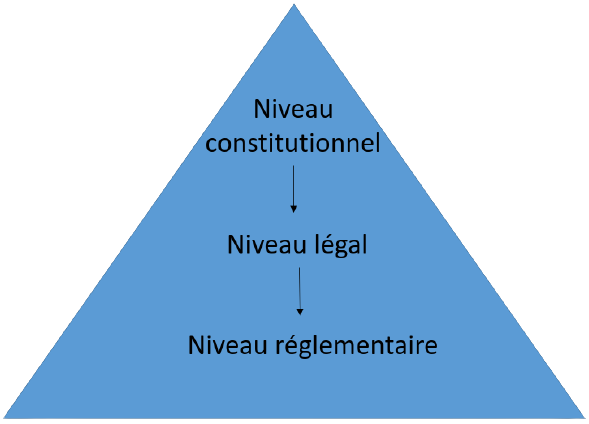
\includegraphics[scale=0.275]{pyramide_des_normes}
    \centering
\end{figure}

\underline{Subtilités de la pyramide des normes :}
\begin{itemize}
\item \textcolor{red}{Collocation} dans un même niveau (ex : lois, décrets et ordonnances)
\item \textcolor{red}{Hiérarchisation} dans un même niveau (ex : lois et décrets > ordonnances)
\end{itemize}

\subsection{Protection juridictionnelle du citoyen}
Les citoyens doivent avoir accès au juge pour réclamer une sanction.

\newpage
\chapter{Leçon 3 : La personne}

\section{Introduction}

\begin{itemize}
    \item Personne : sujet de droit
    \item 2 types :
    \begin{itemize}
        \item Physique
        \item Morale
    \end{itemize}
\end{itemize}

\section{La notion de personne}
\begin{itemize}
    \item Définition : titulaire de droits et d'obligations dans un ordre juridique
    \item 2 remarques :
    \begin{itemize}
        \item Personne : destinataire primaire et secondaire de la règle de droit
        \item Personne : "fiction juridique"
        \begin{itemize}
            \item Pas une réalité naturelle
            \item Ordre juridique qui décide qui est ou non personne (ex : droit international : états = personnes)
        \end{itemize}
    \end{itemize}
\end{itemize}

\subsection{Conséquences de la personnalité juridique}

\begin{enumerate}
    \item \textcolor{red}{Capacité de jouissance} : être titulaire de droits et obligations
    \begin{itemize}
        \item Exceptions : impossibilité d'élire et d'être élu des mineurs et l'indignité successorale en cas d'assassinat.
    \end{itemize}
    \item \textcolor{red}{Capacité d'exercice} : pouvoir exercer ses droits et obligations (autonome)
    \begin{itemize}
        \item Personnes physique majeure : capacité générale d'exercice
        \item Statuts de protection : capacité limitée d'exercice (ex : mineurs, statut protégé)
    \end{itemize}
\end{enumerate}

\section{La personne physique}

\begin{enumerate}
    \item Notion d'\textcolor{red}{être humain}
    \item Pour être une personne physique : Enfant \textcolor{red}{né vivant et viable}.
    \item Un fœtus n'est donc pas une personne physique dans le sens juridique du terme. Pourtant, dans certains cas, on considère l'acquisition de la personnalité juridique au moment de la conception.
    \item On perd sa personnalité juridique au moment du \textcolor{red}{décès} (mort cérébrale).
    \item Le \textcolor{red}{mineur} n'a \textcolor{red}{pas de capacité d'exercice} (sauf émancipation). Ce sont ses parents qui exercent par leur autorité parentale. Cette autorité leur donne aussi le droit de déterminer les orientations de vie de leur enfant. \\
    $\Rightarrow$ Modalités d'exercice de l'autorité parentale :
    \begin{enumerate}
        \item Parents vivent ensemble :
        \begin{itemize}
            \item Exercice conjoint de l'autorité
            \item Si on prend une décision : Présomption d'accord.
        \end{itemize}
        \item Parents séparés :
        \begin{itemize}
            \item Pareil mais exceptions :
            \begin{itemize}
                \item Chacun peut prendre des décisions éducatives.
                \item Peut garde exclusif donnée par le tribunal des familles.
             \end{itemize} 
        \end{itemize}
    \end{enumerate}
    \item Il y a de plus en plus d'exceptions à l'incapacité d'exercice du mineur.
\end{enumerate}

\section{La personne morale}

\begin{itemize}
    \item Entité constituée d'un ensemble de personnes (physiques ou morales) à laquelle le droit attribue une personnalité juridique.
    \item conséquences :
    \begin{itemize}
        \item Droit de jouissance.
        \item Patrimoine \textcolor{red}{propre} = distinct de ses membres.
    \end{itemize}
    \item Il existe 2 types de personnes morales :
    \begin{enumerate}
        \item De droit publique (SPF, communes, ...)
        \item De droit privé (Résiduaire, tout le reste)
        \begin{enumerate}
            \item Limites à la capacité de jouissance "\textcolor{red}{principe de spécialité}"
            \begin{itemize}
                \item Pas d'acte en dehors du cadre légal (code des sociétés)
                \item Ex. : ASBL ne peut pas faire de profit.
            \end{itemize}
            \item Spécialité statuaire : 
            \begin{itemize}
                \item Statut = acte constitutif d'une société
                \item Objet social = ce que fait la société
            \end{itemize}
        \end{enumerate}
    \end{enumerate}
\end{itemize}

\subsection{Classification des personnes morales de droit privé}

\begin{enumerate}
    \item Société :
    \begin{itemize}
        \item Notion :
        \begin{itemize}
            \item Associés (apport numéraire ou en nature)
            \item Créée pour procurer un avantage patrimonial
        \end{itemize}
    \end{itemize}
    \item Associations (ASBL ou AISBL) :
    \begin{itemize}
        \item Notion :
        \begin{itemize}
            \item \textcolor{red}{Membres}
            \item Exercent \textcolor{red}{une activité} formant l'objet de l'association.
            \item Dans un \textcolor{red}{but désintéressé}\\
            $\Rightarrow$ Peut distribuer un avantage patrimonial si dans un but désintéressé (ex. : Lutte contre le précarité)
        \end{itemize}
    \end{itemize}
    \medskip
    \item Fondations :
    \begin{itemize}
        \item Notion :
        \begin{itemize}
            \item Fondateurs
            \item Affectent un patrimoine.
            \item Réalisation d'un but désintéressé (philanthropie)
        \end{itemize}
    \end{itemize}
\end{enumerate}

\subsection{Capacité d'exercice des personnes morale}

\begin{itemize}
    \item Puisque les personnes morales sont des fictions juridiques, elles doivent agir par des \textcolor{red}{organes}.
    \item Notion d'organe : entité \textcolor{red}{agissant au nom} de la personne morale.
    \item Conséquence : organe engage la société pour les actes juridiques accomplis en cette qualité d'organe (ex. :  achat de biens, assemblée générale, conseil d'administration, ...).
\end{itemize}

\newpage
\chapter{Leçon 4 : Les droits subjectifs et patrimoines}

\section{Le droit subjectif}

\begin{itemize}
    \item Définition : \textcolor{red}{prérogative} conférée à une personne déterminée sur la base d'une règle de droit et faisant l'objet d'une protection juridique. \\
    \underline{Exemple : achat d'une voiture :}
	\item Conséquences
    \begin{itemize}
        \item Acheteur = titulaire de droit subjectif (propriété).
        \item Droit de propriété dans la loi $\rightarrow$ protégé par les juges.
    \end{itemize}
    \item 2 catégories :
    \begin{itemize}
        \item Patrimoniaux $\rightarrow$ valeur économique (propriété, ...)
        \item Extra-patrimoniaux $\rightarrow$ pas de valeur économique (droit à la vie, ...)
    \end{itemize}
\end{itemize}

\subsection{Droits extra-patrimoniaux}

\begin{itemize}
	\item Droits inhérents à la personne \\
	$\Rightarrow$ pas évaluable en argent, inaliénable.\\
	\textcolor{red}{\warning} Parfois indirectement évaluable en argent (alimentaire).
	\item 6 caractéristiques :
	\begin{enumerate}
		\item \textcolor{red}{Hors le commerce} : pas d'appropriations privée.
		\item \textcolor{red}{Inaliénable} : pas susceptible de vente.
		\item \textcolor{red}{Indisponible} : pas être l'objet d'un acte juridique (pas de location, échange, ...).\\
		$\Rightarrow$ tempérament : mannequina, sadomasochisme.
		\item \textcolor{red}{Imprescriptible} : pas d'acquisition ou de perte avec le temps (ex. : divorce).\\
		$\Rightarrow$ tempérament : droite de réponse, délai de 3 mois.
		\item \textcolor{red}{Absolus} : même par l'état.
		\item \textcolor{red}{Universels} : reconnus à toute personne.\\
		$\Rightarrow$ tempérament : mineurs.
	\end{enumerate}
	\item 2 catégories :
	\begin{enumerate}
		\item Droits de la personnalité :
		\begin{itemize}
			\item Constituant l'individualité.
		\end{itemize}
		\item Droits fondamentaux :
		\begin{itemize}
			\item Dimension verticale (\textcolor{red}{État vs particulier}).
			\item Dimension horizontale (\textcolor{red}{particulier vs particulier}).
		\end{itemize}
	\end{enumerate}
\end{itemize}

\subsection{Droits patrimoniaux}

\begin{itemize}
	\item 5 caractéristiques :
	\begin{enumerate}
		\item \textcolor{red}{Dans le commerce}
		\item \textcolor{red}{Aliénable} : susceptible de vente.
		\item \textcolor{red}{Disponible} : le titulaire peut en disposer (vente).
		\item \textcolor{red}{Transmissible} : héritable.
		\item \textcolor{red}{Prescriptible} :
		\begin{itemize}
			\item L'écoulement du temps peut permettre d'\textcolor{red}{acquérir} un droit patrimonial.
			\item L'écoulement du temps peut faire \textcolor{red}{perdre} un droit patrimonial.
		\end{itemize}
	\end{enumerate}
\end{itemize}

\subsubsection{Catégorisation}

\begin{enumerate}
	\item Droit de créance : un \textcolor{red}{créancier} peut exiger d'une autre (\textcolor{red}{débiteur} l'accomplissement d'une prestation.
	\begin{enumerate}
		\item Effet relatif : débiteur seulement redevable au créancier.
		\item Peut prendre la forme de :
		\begin{itemize}
			\item Donner (\textit{dare})
			\item Faire (\textit{facere})
			\item Ne pas faire (\textit{non facere})
		\end{itemize}
	\end{enumerate}
	\item Droit réel : permet à son titulaire de directement utiliser, jouir ou disposer d'une chose.
	\begin{itemize}
		\item \textcolor{red}{Pas entre personnes}.
	    \item \textcolor{red}{Opposable} à tous (\textit{erga omnes} : peut en exiger le respect.
	    \item Nombre \textit{limité} par la loi (\textit{numorus clousus})
	    \item 2 sortes :
	    \begin{itemize}
	    	    \item Principaux : \textcolor{red}{existence propre} et ont une \textcolor{red}{utilité}.
	    	    \begin{itemize}
	    	    	    \item 3 prérogatoires (utilisations) :
	    	    	    \begin{itemize}
	    	    	    	    \item \textcolor{red}{Usus} : utiliser la chose.
	    	    	    	    \item \textcolor{red}{Fructus} : recueillir les fruits qu'elle produit (\textcolor{red}{naturel} (générés naturellement), \textcolor{red}{industriel} (générés par le travail : récolte d'un champ, civil (loyer), ...)).
	    	    	    	    \item \textcolor{red}{Abusus} : disposer librement de la chose (\textcolor{red}{juridique} (vente/échange, ...), \textcolor{red}{matériel} (détruire))\\
	    	    	    	    \textcolor{red}{\warning} Seul l'abus permet de prélever les produits (revenus qui entament la substance de la chose (ex : minerai)).
	    	    	    	    \item Le droit de propriété est le seul à combiner les 3 prérogatives.
	    	    	    	    \item Autres droits réels principaux : usage, habitation, usufruit emphytéose, servitude et superficie.
	    	    	    	    \item Ils sont dit "\textcolor{red}{démembrés}", confèrent une ou deux des trois prérogatives.
	    	    	    \end{itemize}
	    	    \end{itemize}\smallskip
	    	    \item Droits réels accessoire :
	    	    \begin{itemize}
	    	    	    \item Pas d'existence propre.
	    	    	    \item Dépend toujours de la créance qu'ils garantissent.\\
	    	    	    $\rightarrow$ But : protéger le créancier de l'insolvabilité.
	    	    	    \item 2 droits :
	    	    	    \begin{enumerate}
	    	    	    	    \item Gage (meubles, objets) : sert à garantir un "prêt".
	    	    	    	    \item Hypothèque (immeuble)\\
	    	    	    	    $\rightarrow$ \textcolor{red}{Droit de préférence} du gagiste ou de la banque : donne la priorité en cas de vente.
	    	    	    \end{enumerate}
	    	    \end{itemize}
	    \end{itemize}
	\end{itemize}
\end{enumerate}

\subsection{Le droit intellectuel}

Confère la maîtrise des créations intellectuelles à son titulaire.

\section{Le patrimoine}

\begin{itemize}
	\item Définition : entité abstraite constituée de l'\textcolor{red}{ensemble} des \textcolor{red}{droits} et \textcolor{red}{obligations} patrimoniaux appartenant à une personne.
	\item Il s'agit d'une \textcolor{red}{universalité de droit}, c'est une abstraction.
	\item Possède un actif et un passif (dette et possessions).
	\item Fonction de garantie :\\
	$\rightarrow$ But : garantir l'exécution des obligations du débiteur par des saisies si insolvabilité.
	\item 5 caractéristiques du patrimoine :
	\begin{enumerate}
		\item \textcolor{red}{Attribut de la personnalité} (attaché à une personne).
		\item \textcolor{red}{Indivisible} : impossible de fractionner ou additionner les patrimoines.\\
		$\rightarrow$ tempérament : patrimoine d'affectation (ex. : mariés), création d'une personne moral.
		\item \textcolor{red}{Inaliénable}
		\item \textcolor{red}{Disparition par confusion lors du décès de son titulaire}
		\begin{itemize}
			\item Contenu transmis aux héritiers
			\item 3 types d'héritiers :
			\begin{itemize}
				\item Ayants cause universel : reçoit tout.
				\item Ayants cause à titre universel : reçoit une partie.
				\item Ayants cause à titre particulier : reçoit un ou plusieurs biens et droits déterminés par un testament.
			\end{itemize}
		\end{itemize}
		\item \textcolor{red}{Gage commun des créanciers} : possibilité de saisie en cas d'insolvabilité.
	\end{enumerate}
\end{itemize}

\newpage
\chapter{Leçon 6 : Le contrat}

\section{La formation du contrat}

\subsection{Introduction}

Contrat = substrat des relations sociales.

\subsection{Notion de Contrat}

\begin{itemize}
	\item Définition : \textcolor{red}{accord de volonté} visant à produire des \textcolor{red}{effets juridiques} (créer, modifier, transmettre ou étendre des droits et obligations).
	\item Contrat : opération simple ou complexe (achat de journal ou de maison).
	\item Naissance du contrat : rencontre de \textcolor{red}{2 volontés} = contrat. Il peut y avoir des \textcolor{red}{discordes} entre les volontés : acheteur peut recouvrir aux \textcolor{red}{vices de consentements} pour l'annuler.
	\item \textcolor{red}{Règles supplétives} très importante (règle sauf si on décide autre chose).
    \item Contrat formé par une \textcolor{red}{offre} et une \textcolor{red}{acceptation}.
    \item Si les \textcolor{red}{éléments essentiels} ne sont pas évoqués (close/prix) il ne s'agit pas d'un contrat au sens \textcolor{red}{juridique}, mais d'une invitation à rentrer en \textcolor{red}{pourparlers}.
\end{itemize}

\subsection{Typologie des contrats}

\begin{enumerate}
	\item Contrats \textcolor{red}{synallagmatiques} : les \textcolor{red}{2 parties} reçoivent des obligations (vente, bail).
	\item Contrats \textcolor{red}{unilatéraux} : \textcolor{red}{une seule partie} reçoit des obligations (prêt, caution).
	\item Contrats \textcolor{red}{consensuels} : formés par un échange de consentement (vente, mandat).
	\item Contrats \textcolor{red}{réels} : formés par la remise d'une chose (prêt).
	\item Contrats \textcolor{red}{solennels} : formés par l'accomplissement d'une forme bien définie (donation).
	\item Contrats \textcolor{red}{nommés} : réglés par des dispositions juridiques (la vente).
	\item Contrats \textcolor{red}{innomés} : pas réglés par des dispositions juridiques (leasing). Dépend de ce qui est mis dans le contrat.
	\item Contrats conclus \textcolor{red}{intuitu personae} : Si la personne avec qui le contrat est passé est importante\\
	$\rightarrow$ Conséquence : Exécution personnelle du débiteur.\\
    $\rightarrow$ Conséquence : Mort, faillite ou incapacité entraine la dissolution du contrat.
    \item Contrats à titre \textcolor{red}{onéreux} : contrats en échange d'une contrepartie (vente).
    \item Contrats à titre \textcolor{red}{gratuit} : contrats purement altruiste (don.
    \bigskip\medskip
    \item Contrats entre personnes privées, entre entreprises et de consommation :
    \begin{itemize}
        	\item si personnes $\rightarrow$ code civil
        	\item si entre entreprise $\rightarrow$ code civil et code de droit économique.
        	\item si contrat de consommation $\rightarrow$ code civil, code de droit économique et droit de la consommation.
    \end{itemize}
\end{enumerate}

\subsection{Les principes}

\begin{itemize}
	\item Principes d'\textcolor{red}{autonomie de la volonté} (ce qu'on veut et avec qui on veut) $\rightarrow$ Moteur de créativité
	\begin{itemize}
		\item Droit de \textcolor{red}{respecter l'ordre public} et les \textcolor{red}{lois impératives} (ex. : de trafic de drogue (nullité absolue) ou de bail à ferme (nullité relative)).
		\item Le \textcolor{red}{contenu} du contrat parfois \textcolor{red}{imposé} par le législateur (ex. : assurance voiture).
		\item Lien entre \textcolor{red}{autonomie} et \textcolor{red}{conditions générales} :
		\begin{itemize}
			\item Les conditions générales définissent le \textcolor{red}{contenu} du contrat et \textcolor{red}{règlent certains problèmes} (indemnités en cas de non payement, etc.).
			\item Pour qu'elles soient \textcolor{red}{opposables}, les conditions générales doivent avoir été \textcolor{red}{lues} et \textcolor{red}{acceptées} par le contractant (signature ou en ne réagissant pas (tacitement)).
		\end{itemize}
		\item Il y a aussi des moyens de \textcolor{red}{protéger} le consommateur (\textcolor{red}{partie faible}) contre les causes abusives :
		\begin{itemize}
			\item Clause qui crée un \textcolor{red}{déséquilibre} droit/obligations du consommateur et d'une entreprise (engagement irrévocable du consommateur ou réserver à l'entreprise le droit de modifier les caractéristiques du produit).\\
			$\rightarrow$ toute clause abusive est \textcolor{red}{interdite} et \textcolor{red}{nulle}.
		\end{itemize}
	\end{itemize}
	\item Principe du \textcolor{red}{consensualisme}
	\begin{itemize}
		\item Demande juste le \textcolor{red}{consentement} des parties, sans besoin de forme.\\
		$\rightarrow$ Sauf pour les contrats \textcolor{red}{solennels} et \textcolor{red}{réels}.
		\item formalisme de protection : \textcolor{red}{formalités} ou \textcolor{red}{mentions} obligatoires pour protéger le consommateur.
		\item formalisme probatoire : le législateur impose certaines règles pour rendre le contrat valable en justice (le contrat est quand même valide).
	\end{itemize}
	\item Principe de la \textcolor{red}{convention-loi}
	\begin{itemize}
		\item Chaque partie \textcolor{red}{respecte ses engagements}.
		\item Le contrat ne peut être modifié que d'\textcolor{red}{accord commun}.\\
		$\rightarrow$ Un juge ne peut pas modifier le contrat. \textit{"Le contrat est la loi des parties."}\\
		$\rightarrow$ Tempérament : droit de rétraction.
	\end{itemize}
	\bigskip\medskip
	\item Principe de \textcolor{red}{bonne foi} et de l'\textcolor{red}{abus de droit}.
	\begin{itemize}
		\item Bonne foi = respect de la correction et loyauté lors de la formation et exécution du contrat.
		\begin{itemize}
			\item La loyauté impose de donner des informations (\textcolor{red}{complétives}).
			\item Faire preuve de modération dans l'application des clauses contractuelles (\textcolor{red}{modératrice}).
		\end{itemize}
		\item Abus de droit = exercice d'un droit d'une manière qui \textcolor{red}{excède les limites} de l'exercice normal de ce droit pas une personne prudente.
		\begin{itemize}
			\item Critères de l'interdiction de l'abus de droit :
			\begin{itemize}
				\item Intention de \textcolor{red}{nuire}.
				\item Sans intérêt ou de \textcolor{red}{façon disproportionnée} (exercice > dommage).
				\item \textcolor{red}{Détournement} de la fonction légale initiale.
				\item Liste non exhaustive (cas de la "\textcolor{red}{rechtsverwerking}" (ex. : réclamer des intérêts 5 ans plus tard).
			\end{itemize}
		\end{itemize}
	\end{itemize}
	\item Principe de la \textcolor{red}{relativité du contrat}
	\begin{itemize}
		\item Un contrat est personnel entre les contractants.\\
		$\rightarrow$ Exception 1 : \textcolor{red}{La stipulation pour autrui} : Les parties s'accordent pour faire naitre à charge d'un \textcolor{red}{promettant}, un droit au profit d'une \textcolor{red}{tierce personne} (ex. : contrat d'assurance-vie).\\
		$\rightarrow$ Exception 2 : \textcolor{red}{L'action directe} : Hypothèse où un tiers peut se prévaloir d'une créance issue d'un contrat auquel il n'est \textcolor{red}{pas partie} (\textcolor{red}{origine légale}) (ex. : victime d'un accident de la route).
	\end{itemize}
\end{itemize}

\subsection{Formation dynamique du contrat}

\begin{itemize}
	\item Les \textcolor{red}{pourparlers} (négociation)
	\begin{itemize}
		\item Tant que les parties sont en pourparlers, il n'y a pas de contrat.
		\item 2 effets juridiques :
		\begin{itemize}
			\item Rupture \textcolor{red}{fautive} des pourparlers (faire croire qu'on va s'engager alors que non)\\
			$\rightarrow$ \textcolor{red}{indemniser} la victime des frais de négociation.
			\item \textcolor{red}{Interprétation} du contrat (faire attention aux interprétations des documents échangés).
		\end{itemize}
	\end{itemize}
	\item Les \textcolor{red}{accord préalables} au contrat définitifs
	\begin{itemize}
		\item L'\textcolor{red}{avant contrat} : contrat préparatoire (confidentialité)
		\item \textcolor{red}{Lettres d'intention} : lettre manifestant la volonté de conclure (pas un contrat), sert à renforcer la bonne foi.
		\item \textcolor{red}{Accords de principe} : prévoir un accord sur les points essentiels du contrat, le reste est encore à voir ultérieurement.\\
		$\rightarrow$ Si pas d'accord au final, \textcolor{red}{règles supplétives}.
	\end{itemize}
\end{itemize}

\subsection{Les conditions de la validité du contrat (formation statique}

\begin{itemize}
	\item Le consentement : les parties doivent avoir la volonté de s'engager en droit.\\
	$\rightarrow$ Pas valable en cas d'\textcolor{red}{erreur} : croire que ce qui est faux est vrai (ex. : achat d'un tableau).
	\begin{itemize}
		\item \textcolor{red}{Erreur-obstacle} : tellement grave que pas de consentement.
		\begin{enumerate}
			\item Erreur de \textcolor{red}{nature} (\textit{in negotio}) (vente/location).
			\item Erreur d'\textcolor{red}{objet} (\textit{in corpore}) (pas l'objet qu'on pensait).
		\end{enumerate}
		\item \textcolor{red}{Erreur sur la substance} : Erreur sur une qualité qui était importante
		\begin{itemize}
			\item Doit pouvoir prouver que le cocontractant \textcolor{red}{connaissait la qualité}.
			\item Doit pouvoir prouver que l'erreur est \textcolor{red}{excusable} (fait d'un homme raisonnable).\\
			$\rightarrow$ Sanction : nullité relative.\\
			$\rightarrow$ Sanction : dommage et intérêts.
		\end{itemize}
	\end{itemize}
	$\rightarrow$ Pas valable en cas de \textcolor{red}{dol} :
	\begin{itemize}
		\item Manœuvre \textcolor{red}{frauduleuse}.
		\item Manœuvre \textcolor{red}{déterminante} du consentement.
		\item Manœuvre doivent \textcolor{red}{émaner du cocontractant}.\\
		$\rightarrow$ 2 remarques :
		\begin{itemize}
			\item Erreur ne doit pas forcément être excusable.
			\item Dol par silence = Dol.
		\end{itemize}
		$\rightarrow$ Sanction : \textcolor{red}{dol principal} (pas déterminant, aurait quand même acheté).
		\begin{itemize}
			\item Réduction du prix par dommage et intérêts.
		\end{itemize}
	\end{itemize}
	$\rightarrow$ Pas valable en cas de \textcolor{red}{violence} :
	\begin{itemize}
		\item \textcolor{red}{Victime} = cocontractant ou proche.
		\item \textcolor{red}{Auteur} = cocontractant ou tiers.
		\item \textcolor{red}{Déterminante}.
		\item \textcolor{red}{Nature} : réelle, physique ou morale et doit être suffisamment forte.
		\item \textcolor{red}{Injuste ou illicite} : en dehors des autorités morales ou économiques.\\
		$\rightarrow$ Sanction : violence déterminante
		\begin{itemize}
			\item Nullité relative.
			\item Dommage et intérêts.
		\end{itemize}
		$\rightarrow$ Sanction : violence incidente
		\begin{itemize}
			\item Dommage et intérêts.
		\end{itemize}
	\end{itemize}
	$\rightarrow$ Pas valable en cas de \textcolor{red}{lésion} :
	\begin{itemize}
		\item Consiste en un \textcolor{red}{déséquilibre} entre les prestations des parties existantes au moment de la conclusion.
		\item Que dans des cas particuliers.
		\begin{itemize}
			\item Lésion \textcolor{red}{simple} :
			\begin{itemize}
				\item Avec un mineur
				\item De plus d'un quart en matière de partage.
				\item De plus de 7/12 pour la vente d'un immeuble (protège le vendeur, pas l'acheteur).
			\end{itemize}
			$\rightarrow$ Sanction :
			\begin{itemize}
				\item Nullité absolue.
			\end{itemize}
			\item Lésion \textcolor{red}{qualifiée} : abus de faiblesse de l'âge, de l'inexpérience ou des passions de la victime.
			$\rightarrow$ Sanction :
			\begin{itemize}
				\item Nullité relative.
			\end{itemize}
		\end{itemize}
	\end{itemize}
	\item L'\textcolor{red}{objet}
	$\rightarrow$ L'objet doit être dans le commerce et passible.
	\begin{itemize}
		\item Si la loi dit qu'une chose n'est \textcolor{red}{plus dans le commerce} (ex. : viande pourrie), elle ne peut pas faire l'objet d'un contrat.
		\item Si la chose est \textcolor{red}{impossible à vendre} (ex. : la lune), elle ne peut pas faire l'objet d'un contrat.
	\end{itemize}
	$\rightarrow$ L'objet doit être déterminé ou déterminable.
	\begin{itemize}
		\item \textcolor{red}{Déterminé} s'il y a assez de détails permettant de définir l'étendue des prestations des parties.
		\item \textcolor{red}{Déterminable} si elle contient suffisamment d'\textcolor{red}{éléments objectifs} permettant de définir les prestations des parties (ex. : achat d'actions au prix à telle date).
		\item Imprécisions de l'objet réglé par les \textcolor{red}{usages professionnels} et les \textcolor{red}{règles de l'art}.
		\item Il est possible qu'un tiers ou une des partie détermine l'objet (ex. : avocat déterminant sa marche à suivre). Le juge peut en contrôler la \textcolor{red}{bonne foi} ou se baser sur les \textcolor{red}{règles applicables} à une profession pour contrôler cette décision.
		\item Il est également possible d'insérer une \textcolor{red}{clause de modification unilatérale} du contrat. Cela permet à une partie de modifier le contrat en cous. Dans ce cas, il est bon d'accorder une \textcolor{red}{clause de résiliation}.
		\item Les choses futures (ex. : récoltes de l'année prochaine) peuvent être l'objet d'un contrat si elles sont déterminées ou déterminables.
	\end{itemize}
	\item La \textcolor{red}{cause} : Le pourquoi (raison de validité) du contrat.
	\begin{itemize}
		\item Un contrat \textcolor{red}{dépourvu} de cause est considéré nul.
		\item Si la cause est \textcolor{red}{illicite}, le contrat est nul.
		\item Double acception de la cause.
		\begin{itemize}
			\item Acception \textcolor{red}{objective} (cause = contrepartie du cocontractant).
			\item Acception \textcolor{red}{subjective} (cause = mobiles déterminants).
		\end{itemize}
	\end{itemize}
	\item La \textcolor{red}{capacité} : Il faut être juridiquement capable de contracter.
\end{itemize}

\subsection{Ordre public, bonnes mœurs et les lois impératives}

\begin{itemize}
	\item Ordre public : dispositions qui ont trait aux intérêts essentiels de l'état ou qui fixent les bases juridiques de l'\textcolor{red}{ordre économique} ou \textcolor{red}{moral} $\rightarrow$ Intérêt \textcolor{red}{général} (nullité absolue)
	\item Impérativité : dispositions qui ont trait aux \textcolor{red}{intérêts privés} $\rightarrow$ la \textcolor{red}{partie faible} (nullité relative).
\end{itemize}

\section{L'exécution des obligations ainsi que quelques cas spéciaux}

\subsection{L'exécution}

\begin{itemize}
	\item Le \textcolor{red}{paiement} est un acte juridique unilatéral qui constitue l'exécution d'une \textcolor{red}{obligation}.
	\begin{itemize}
		\item Paiement $\neq$ un contrat (pas besoin d'accord).
		\item Le créancier ne \textcolor{red}{peut pas refuser} le payement par un \textcolor{red}{tiers} ou par un \textcolor{red}{agent d'exécution} (à part pour les contrats intiutu personae)
		\item Le \textcolor{red}{bénéficiaire} doit être le \textcolor{red}{créancier} ou un \textcolor{red}{mandataire}. Ce mandataire doit être fait à une \textcolor{red}{personne capable} de le recevoir. Une \textcolor{red}{ratification} (signature) peut être faite en cas de payement non valable (appropriation d'un acte étranger).
		\item Le payement est \textcolor{red}{valable seulement si} il porte sur l'\textcolor{red}{objet initialement prévu}\\
		$\rightarrow$ Payement \textcolor{red}{partiel} n'est pas libératoire.
		$\rightarrow$ Les parties peuvent faire une \textcolor{red}{dation en paiement} pour modifier l'objet du paiement (sert à convenir que la \textcolor{red}{remise} d'une \textcolor{red}{chose différente} est \textcolor{red}{libératoire}).
	\end{itemize}
	\item La \textcolor{red}{responsabilité contractuelle} : s'il y a \textcolor{red}{manquement} (ex. : pas de livraison, pas de loyer) $\rightarrow$ violation \textcolor{red}{convention-loi}.
	\begin{itemize}
		\item Le créancier doit d'abord définir l'\textcolor{red}{étendue} des obligations du débiteur.
		\begin{itemize}
			\item \textcolor{red}{Obligation de résultat} : responsable si \textcolor{red}{résultat} pas obtenu (sauf force majeure).
			\item \textcolor{red}{Obligation du moyen} : responsable si le débiteur ne s'est pas \textcolor{red}{comporté} comme un homme normalement prudent et diligent.\\
			$\rightarrow$ Le \textcolor{red}{juge} décide de l'\textcolor{red}{intensité} de l'obligation (dépend de la \textcolor{red}{complexité}) (ex. : appel vs opération).
		\end{itemize}
		\item On peut insérer au contrat une \textcolor{red}{clause d'exonération de responsabilité} pour limiter ou supprimer la responsabilité contractuelle du débiteur en cas d'inexaction.
		\begin{itemize}
			\item Limite 1 : On ne peut s'exonérer de \textcolor{red}{son dol}.
			\item Limite 2 : Interdiction de \textcolor{red}{vider l'obligation de son objet} (on doit quand même s'exécuter).
		\end{itemize}
		\item Événements perturbateurs (événements excusant le débiteur).
		\begin{itemize}
			\item \textcolor{red}{Force majeure} : événement imprévisible et inévitable rendant l'exécution de l'obligation impossible.
			\begin{itemize}
				\item \textcolor{red}{Définitive} : dissolution du contrat.
				\item \textcolor{red}{Temporaire} : suspension jusqu'à la fin de la force majeure.
			\end{itemize}
			\item L'\textcolor{red}{imprévision} : événement imprévisible et non imputable au débiteur qui bouleverse \textcolor{red}{l'économie contractuelle} (rend plus difficile).
			\begin{itemize}
				\item Conséquence : révision.
				\item Statut incertain (pas reconnu par tous).
			\end{itemize}
		\end{itemize}
	\end{itemize}
\end{itemize}

\subsection{L'inexécution}

\begin{enumerate}
	\item \textcolor{red}{Mise en demeure} : dernière sommation obligatoire avant des poursuites judiciaires.
	\begin{itemize}
		\item Cas où elle n'est pas requise.
		\begin{itemize}
			\item Contrat le \textcolor{red}{prévois}.
			\item Quand c'est \textcolor{red}{inutile} (ex. : date passée).
			\item \textcolor{red}{Débiteur} a fait savoir qu'il \textcolor{red}{ne le ferait pas}.
		\end{itemize}
		\item \textcolor{red}{Pas de force} requise.
		\item Aucune formule sacramentelle, ce qui est important c'est d'être clair et non équivoque.
		\item La mise en demeure fait courir les \textcolor{red}{intérêts moratoires} (de retard = 8\%/an).
		\item Elle \textcolor{red}{déplace les risques} (énonce les responsabilités du fautif (ex. : cheval mort après achat)).
	\end{itemize}
	\item Réclamer l'\textcolor{red}{exécution en nature}
	\begin{itemize}
		\item Demande au juge d'obliger le débiteur à exécuter la prestation convenue.
		\item Garantir le respect par \textcolor{red}{voie d'astreinte} : somme ) payer par jour après la date déterminée dans son jugement.
	\end{itemize}
	\item \textcolor{red}{Dommages et intérêts}
	\begin{itemize}
		\item À réclamer quand nature est \textcolor{red}{abusive} ou quand cela ne \textcolor{red}{suffit pas à réparer} le dommage.
		\item Somme d'argent destinée à faire comme si le débiteur ne s'était pas mal exécuté.
		\item Synonyme de "\textcolor{red}{engager la responsabilité contractuelle}".
		\item 3 conditions :
		\begin{itemize}
			\item \textcolor{red}{Faute} contractuelle.
			\item Existence de \textcolor{red}{dommage}.
			\item \textcolor{red}{Lien causal} entre la faute et le dommage.
		\end{itemize}
	\end{itemize}
	$\rightarrow$ Pour éviter tout ça, on peut intégrer une \textcolor{red}{clause pénale} : mettre dans le contrat une comme d'argent à payer en cas d'inexécution.
	\begin{itemize}
		\item \textcolor{red}{Avantage} : pas de preuve du dommage à fournir.
		\item \textcolor{red}{Limites} : fonction indemnitaire, interdiction des clauses excessives. Pas de fonction punitive.
	\end{itemize}
	\item \textcolor{red}{Résolution judiciaire} : anéantissement d'un contrat par le juge en raison d'une faute du débiteur.
	\begin{itemize}
		\item Conditions :
		\begin{itemize}
			\item \textcolor{red}{Mise en demeure}.
			\item Contrat \textcolor{red}{synallagmatique}.
			\item Manquement \textcolor{red}{grave} $\rightarrow$ déterminé par le juge.
			\item Intervention du \textcolor{red}{juge}.
		\end{itemize}
		\item Effets :
		\begin{itemize}
			\item Dissolution rétroactive du contrat : on revient à la situation pré contractuelle.
			\item Dommages et intérêts complémentaires à la résolution possible en plus.
		\end{itemize}
	\end{itemize}
	\item L'\textcolor{red}{exception d'inexécution} (ENAC)
	\begin{itemize}
		\item Suspension de ses obligations tant que le cocontractant n'exécute pas les siennes. $\rightarrow$ Moyen de pression et de protection.
		\item Conditions d'application :
		\begin{enumerate}
			\item Contrat \textcolor{red}{synallagmatique}.
			\item Contrat \textcolor{red}{exigible} (pas de délai).
			\item Créance \textcolor{red}{certaine} mais pas \textcolor{red}{liquide}.
			\begin{itemize}
				\item Certitude : la créance existe (pas contestée).
				\item Liquidité : montant déterminé exactement.
			\end{itemize}
			\item L'\textcolor{red}{excipiens} (celui qui soulève l'inexécution) est de \textcolor{red}{bonne foi}.
			\item Faute contractuelle de \textcolor{red}{gravité suffisante}.
		\end{enumerate}
		\item Effets :
		\begin{itemize}
			\item L'ENAC a un caractère \textcolor{red}{temporaire}.
			\item Si devient définitive, peut se transformer en \textcolor{red}{résolution judiciaire} ou en \textcolor{red}{réduction prix}.
		\end{itemize}
	\end{itemize}
\end{enumerate}

\subsection{La prescription}

\begin{itemize}
	\item Notion de perte de \textcolor{red}{droite patrimonial} par écoulement du \textcolor{red}{temps}.
	\item Toute action personnelle est prescrite de \textcolor{red}{10 ans}.
	\item \textcolor{red}{Citer} son débiteur \textcolor{red}{en justice} réinitialise le délai.
	\item Si le débiteur signe une \textcolor{red}{reconnaissance de dettes}, réinitialise le délai.
	\item \textcolor{red}{Suspension} de la prescription : événement suspendant le cours de la prescription et lorsqu'il disparait, la prescription recommence à courir (\textcolor{red}{minorité)}.
\end{itemize}

\subsection{Les contrats spéciaux}

\begin{itemize}
	\item La \textcolor{red}{vente} :
	\begin{itemize}
		\item Contrat qui transfère la propriété d'un bien contre payement.
		\item Le transfert de propriété s'effectue au moment de l'échange des consentements, pas à la résolution des obligations.
		\item Les obligations du vendeur :
		\begin{enumerate}
			\item Le vendeur doit délivrer une chose conforme.
			\item Le vendeur doit garantir l'acheteur contre les vices cachés\\
			$\rightarrow$ en cas de vice caché, il faut agir dans un bref délai.
			\item Le vendeur doit une garantie d'éviction à l'acheteur (garantir la pleine jouissance, pas de droit d'un tiers sur la chose).
		\end{enumerate}
		\item Les obligations de l'acheteur :
		\begin{enumerate}
			\item L'acheteur doit payer le prix convenu.
			\item Retirer la chose vendue et procéder à son examen attentif.
		\end{enumerate}
	\end{itemize}
	\item Le contrat d'\textcolor{red}{entreprise} (prestation de service)
	\begin{itemize}
		\item Contrat où un entrepreneur s'engage à effectuer un \textcolor{red}{travail intellectuel ou matériel} moyennant un prix.
		\item Obligation de l'entrepreneur : exécuter la \textcolor{red}{prestation} et \textcolor{red}{remettre l'ouvrage} au maitre d'ouvrage.
		\item obligation du maitre d'ouvrage : payer le \textcolor{red}{prix} et \textcolor{red}{collaborer}.
	\end{itemize}
	\item Le \textcolor{red}{mandat} (accomplissement d'acte juridique)
	\begin{itemize}
		\item Transfert de pouvoir d'accomplir en son nom des \textcolor{red}{actes juridiques}.\\
		$\rightarrow$ élément central = la \textcolor{red}{représentation}.
		\item Obligation du mandant
		\begin{itemize}
		 	\item Payer des \textcolor{red}{honoraires} si convenu.
		 	\item \textcolor{red}{Indemniser} le mandataire de ses frais.
		 \end{itemize}
		 \item Obligation du mandataire : \textcolor{red}{accomplir} la mission (responsable de ses fautes envers le mandant), \textcolor{red}{rendre compte} de sa mission, \textcolor{red}{justifier ses frais}.
	\end{itemize}
\end{itemize}

\newpage
\chapter{Leçon 7 : La responsabilité extracontractuelle}

\section{Généralités}
Toute personne doit \textcolor{red}{répondre des fautes} qu'elle a commise.
\begin{itemize}
	\item \textcolor{red}{Civil} (contractuelle et extracontractuelle)
	\item \textcolor{red}{Pénal} (protège l'ordre public)\\
	$\rightarrow$ Relation : faute pénale peut occasionner des \textcolor{red}{dommages à un tiers.}
\end{itemize}

\section{Responsabilité extracontractuelle}
\begin{itemize}
	\item Personne physique ou morale cause des \textcolor{red}{dommages à un tiers} par sa faute.
	\item Objectif : \textcolor{red}{Indemnisation du dommage}.
	\item Il existe aussi des dommages sans fautes/responsabilités = \textcolor{red}{fait générateur}.
\end{itemize}

\section{Cumul des responsabilités (contractuelles et extracontractuelles}
\begin{itemize}
	\item Il est possible d'agir de façon extracontractuelle contre un cocontractant à certaines \textcolor{red}{conditions}. On peut faire ça pour \textcolor{red}{contourner} une clause d'\textcolor{red}{exonération de responsabilité}.
	\begin{itemize}
		\item Conditions : doit pouvoir prouver que le cocontractant a fait un \textcolor{red}{manquement} à une obligation générale de \textcolor{red}{prudence} et que le dommage est outre que celui résultant de la \textcolor{red}{mauvaise exécution du contrat}.
		\item Exception : toujours permis en cas d'infraction pénale.
 	\end{itemize}
\end{itemize}

\section{Éléments constitutifs}
\begin{itemize}
	\item Faute
	\item Dommage
	\item Lien causal
\end{itemize}

\subsection{Faute}
\begin{itemize}
	\item Violation d'une \textcolor{red}{norme de conduite}.
	\begin{itemize}
		\item \textcolor{red}{Disposition légale} sur un comportement.
		\item Violation d'un comportement qu'aurait adopté quelqu'un de \textcolor{red}{prudent et diligent} (appréciation abstraite du \textcolor{red}{bon père de famille}).
	\end{itemize}
	\item Une \textcolor{red}{faute légère} suffit pour engager la responsabilité extracontractuelle.
	\item Pas de distinction entre volontaire et involontaire.
	\item Imputabilité ou comportement libre et conscient :
	\begin{itemize}
		\item \textcolor{red}{Discernement} est-il capable de comprendre les conséquences dommageables (prends en compte les qualités personnelles) ?
		\begin{itemize}
			\item Enfants en bas âge
			\item Troubles mentaux
			\item Perte passagère des facultés mentale
		\end{itemize}
		\item Cause de \textcolor{red}{justification} : circonstances externes (plus de libre arbitre (légitime défense, état de nécessité)).
	\end{itemize}
\end{itemize}

\subsection{Dommage}
\begin{itemize}
	\item \textcolor{red}{Perte} d'un avantage quelconque, ou lésion matérielle ou immatérielle.\\
	\underline{Exemples :}
	\begin{itemize}
		\item \textcolor{red}{Corporel}
		\item \textcolor{red}{Matériel}
		\item \textcolor{red}{Morale}
		\item \textcolor{red}{Économique}
	\end{itemize}
	\item 3 caractères du dommage réparable :
	\begin{enumerate}
		\item \textcolor{red}{Certain} (pas hypothétique ou éventuel)
		\item \textcolor{red}{Légitime} (pas illicite)
		\item \textcolor{red}{Personnel} (victime reçoit le dommage)
	\end{enumerate}
\end{itemize}

\subsection{Lien Causal}
\begin{itemize}
	\item Lien \textcolor{red}{faute/dommage}.
	\item Équivalence des conditions : la faute est a condition du dommage.
	\item Preuve revient à la victime.
	\item On retient toutes les fautes causales.
	\item Si la \textcolor{red}{victime} cause en partie le dommage, sa faute est retenue.
\end{itemize}

\section{Les conséquences de la responsabilité}
\begin{itemize}
	\item Principes de base : \textcolor{red}{indemniser} la victime.
	\begin{itemize}
		\item L'\textcolor{red}{évolution du dommage} se fait de manière concrète. On prend en compte les \textcolor{red}{qualités personnelles} de la victime.
		\item \textcolor{red}{Réparation intégrale} : réparation de tout le dommage causé pour remplacer la victime dans la situation \textcolor{red}{pré-faute}. La réparation ne peut cependant \textcolor{red}{pas enrichir la victime}.
	\end{itemize}
	\item Deux sortes de réparations :
	\begin{itemize}
		\item Réparation en \textcolor{red}{nature} (au sens propre, de manière non pécuniaire)
		\item Réparation par \textcolor{red}{équivalent} (si nature abusive, réparation, par dommage et intérêts)
	\end{itemize}
\end{itemize}

\subsection{Le cas de la pluralité des fautes}
\begin{itemize}
	\item Condamnation \textcolor{red}{in solidum}.
	\item Deux stades :
	\begin{itemize}
		\item \textcolor{red}{Obligation à la dette (auteur-victime}
		\begin{itemize}
			\item \textcolor{red}{Droit d'élection} de la victime : droit de réclamer la réparation intégrale à chaque auteur $\rightarrow$ \textcolor{red}{garantie}.
			\item Mais elle ne peut \textcolor{red}{pas obtenir plus} que son dommage.
		\end{itemize}
		\item \textcolor{red}{Contribution à la dette} (auteur-auteur)
		\begin{itemize}
			\item Action contre le coauteur pour qu'il \textcolor{red}{rembourse sa part}.
			\item \textcolor{red}{Calcul} de sa part : $\frac{\textrm{dommage}}{\textrm{nombre de fautifs}}$.
		\end{itemize}
	\end{itemize}
\end{itemize}

\section{Hypothèses particulières de responsabilité extracontractuelle}

\subsection{Régimes particuliers}
\begin{itemize}
	\item \textcolor{red}{Pères et mères} responsables \textcolor{red}{enfants mineures}
	\begin{itemize}
		\item Parents doivent surveiller et éduquer leurs enfants
		\item Parents payent pour leurs enfants qui sont rarement solvables.
		\item Conditions :
		\begin{itemize}
			\item \textcolor{red}{Mineurs} au moment de la faute.
			\item \textcolor{red}{Parents légaux} (biologiques ou adoptifs).
			\item \textcolor{red}{Faute} ou \textcolor{red}{Acte objectivement illicite} de l'enfant.
			\begin{itemize}
				\item Faute : évaluation de la capacité de discernement de l'enfant $\rightarrow$ Peut mener à ce que la responsabilité personnelle de l'enfant soit également engagée.
				\item Acte objectivement illicite : pas de capacité de discernement, mais aurait été une faute si commise par un adulte.
			\end{itemize}
			\item \textcolor{red}{Dommage} et \textcolor{red}{lien causal}.
		\end{itemize}
	    \item Conséquences :
	    \begin{itemize}
	    	\item Double \textcolor{red}{présomption de faute} des parents (d'\textcolor{red}{éducation} et de \textcolor{red}{surveillance}).
	    	\item Le fait que ce ne soit qu'une présomption permet le caractère \textcolor{red}{réfragable} si les parents démontrent l'absence de faute (surveillance, âge, parcours de vies).
	    \end{itemize}
	\end{itemize}
	\item \textcolor{red}{Maitres et commettants} (employeurs) responsables \textcolor{red}{domestiques et préposés}
	\begin{itemize}
		\item Fondement un peu \textcolor{red}{flou} mais basé sur un \textcolor{red}{aspect économique} (se faire de l'argent sur le dos de ses employés) et \textcolor{red}{pragmatique} (employeur plus solvable).
		\item Conditions :
		\begin{itemize}
			\item Lien de \textcolor{red}{subordination} (ex : contrat de travail)
			\item Faute du \textcolor{red}{préposé}, un \textcolor{red}{dommage} et \textcolor{red}{lien de causalité}.
			\item Faute commise dans le \textcolor{red}{cadre des fonctions}.
		\end{itemize}
		\item Conséquences :
		\begin{itemize}
			\item \textcolor{red}{Pas de présomption} de faute.
			\item \textcolor{red}{Irréfragable}.
		\end{itemize}
		\item Le travailleur n'est responsable que de \textcolor{red}{son dol} ou de sa \textcolor{red}{faute lourde}, faute légère, si \textcolor{red}{habituelle}.
	\end{itemize}
	\item \textcolor{red}{Instituteurs et artisans} responsable \textcolor{red}{élèves et apprentis}
	\begin{itemize}
		\item Fondement : doivent être \textcolor{red}{surveillés}.
		\item Conditions :
		\begin{itemize}
			\item \textcolor{red}{Artisan} et \textcolor{red}{apprentis}.
			\item \textcolor{red}{Instituteur} et \textcolor{red}{élève} (transmission de savoir ou d'éducation).
			\item une faute d'\textcolor{red}{élève}.
			\item \textcolor{red}{Pendant} le temps de la surveillance.
			\item \textcolor{red}{Dommage} et \textcolor{red}{lien causal}.
		\end{itemize}
		\item Conséquence :
		\begin{itemize}
			\item \textcolor{red}{Présomption de faute} de surveillance..
			\item \textcolor{red}{Réfragable}.
			\item Enseignants bénéficient de l'\textcolor{red}{immunité personnelle} de responsabilité civile si \textcolor{red}{employés ou statutaire}.
			\item Possibilité de \textcolor{red}{cumul des responsabilités}.
		\end{itemize}		
	\end{itemize}
	$\rightarrow$ Attention, les parents, instituteurs et artisans peuvent \textcolor{red}{se retirer} la responsabilité s'ils prouvent qu'ils \textcolor{red}{n'ont pu empêcher le fait} $\neq$ les commettants).
\end{itemize}

\subsection{Responsabilité du gardien d'une chose}
\begin{itemize}
	\item On est responsable du dommage que l'on cause, mais aussi celui des \textcolor{red}{choses que l'on a sous la garde}.
	\item Conditions :
	\begin{itemize}
		\item Un \textcolor{red}{gardien} de la chose :
		\begin{itemize}
			\item Celui qui \textcolor{red}{use, jouit} et \textcolor{red}{conserve} la chose.
			\item Notion de fait qui \textcolor{red}{dépend des circonstances} (propriétaire pas toujours le gardien).
		\end{itemize}
		\item Un \textcolor{red}{vice} de la chose :
		\begin{itemize}
			\item Caractéristique \textcolor{red}{anormale} qui risque de causer un dommage.
			\item Remarque : 
			\begin{itemize}
				\item Comparaison avec un \textcolor{red}{modèle de référence}.
				\item Caractère du vice : \textcolor{red}{pas forcément permanent} ni forcément \textcolor{red}{connu du gardien} et peut résulter de l'\textcolor{red}{adjonction d'une chose} à une autre.
			\end{itemize}
		\end{itemize}
	\end{itemize}
	\item Conséquences :
	\begin{itemize}
		\item Responsabilité \textcolor{red}{irréfragable}.
	\end{itemize}
\end{itemize}

\subsection{Responsabilité du fait des animaux}
\begin{itemize}
	\item Fondement : responsable de ses animaux.
	\begin{itemize}
		\item Moral : animal = risque
		\item Pragmatique : animal n'a pas la personnalité juridique.
	\end{itemize}
	\item Condition
	\begin{itemize}
		\item Animal.
		\item Un fait qui cause un dommage.
		\item Gardien : maitrise, direction, et contrôle (pas toujours propriétaire).
	\end{itemize}
	\item Conséquences :
	\begin{itemize}
		\item Responsabilité \textcolor{red}{irréfragable}.
	\end{itemize}
\end{itemize}

\newpage
\chapter{Leçon 12 : Fédéralisme belge}

\section{Perspective historique}

\begin{itemize}
	\item État fédérale : d'autres centres de pouvoir
	\begin{itemize}
		\item \textcolor{red}{3 communautés} :
		\begin{itemize}
			\item Flamande
			\item Française
			\item Germanophone
		\end{itemize}
		\item \textcolor{red}{3 régions} :
		\begin{itemize}
			\item Bruxelles-Capitale
			\item Wallonie
			\item Flandre
		\end{itemize}
	\end{itemize}
\end{itemize}

\subsection{Évolution des Institutions}

\begin{itemize}
	\item Constitution du 7/02/1831:
	\begin{itemize}
		\item État belge (\textcolor{red}{unitaire}) : un seul centre de pouvoir.
	\end{itemize}
	\item 1\up{ère} réforme 1970 :
	\begin{itemize}
		\item Passage au \textcolor{red}{fédéralisme} (création des \textcolor{red}{communautés culturelles})
	\end{itemize}
	\item 2\up{e} réforme 1980 :
	\begin{itemize}
		\item Approfondissement de 1970 : passage aux \textcolor{red}{Communautés}.
		\item Création des \textcolor{red}{régions Wallone} et \textcolor{red}{Flammande}.
	\end{itemize}
	\item 3\up{e} réforme 1988-89 :
	\begin{itemize}
		\item Création de \textcolor{red}{Bruxelles-Capitale}.
		\item Transfert de \textcolor{red}{compétences d'enseignement} aux communautés.
	\end{itemize}
	\item 4\up{e} réforme 1993 :
	\begin{itemize}
		\item Achèvement
		\item Article 1\up{er} de la \textcolor{red}{Constitution} : Belgique = état fédéral.
	\end{itemize}
	\item 5\up{e} réforme 2000-2001
	\begin{itemize}
		\item \textcolor{red}{Transfert de compétences} aux communautés et régions (lois communales et provinciales).
		\item Modifications des institutions Bruxelloises pour \textcolor{red}{protéger les néerlandophones}.
	\end{itemize}
	\item 6\up{e} réforme 2011-14
	\begin{itemize}
		\item Saga BHV "\textcolor{red}{Bx-Halle-Vilvorde}" : réforme arrondissement électoral et judiciaire de BHV.
		\item \textcolor{red}{Transfert de compétences} aux communautés et aux régions.
		\item Nouvelle \textcolor{red}{loi de financement} : 20 milliards d'euros aux entités fédérées.
		\item Réforme du Sénat et de la chambre : \textcolor{red}{Chambre > Sénat}.
	\end{itemize}
\end{itemize}

\section{Le paysage institutionnel belge}
\begin{itemize}
	\item 5 remarques :
	\begin{enumerate}
		\item Terminologie
		\begin{itemize}
			\item État : \textcolor{red}{lois}
			\item Communautés et Régions (Wallonie et Flandre) : \textcolor{red}{décrets}
			\item Région Bruxelles-Capitale et COCOM : \textcolor{red}{ordonnances}
		\end{itemize}
		\item Chaque entité est entièrement \textcolor{red}{compétente dans ses matières}
		\begin{itemize}
			\item Régions : compétences du territoire
			\item Communautés : compétences liées aux personnes
		\end{itemize}
		\item Existence de \textcolor{red}{4 régions linguistiques} (simple délimitations territoriales)
		\begin{itemize}
			\item Française
			\item Néerlandaise
			\item Bilingue (Bx)
			\item Allemande
		\end{itemize}
		\item Chaque entité = exerce sur son territoire
		\begin{itemize}
			\item Régions : territoires
			\item Communautés :
			\begin{itemize}
				\item française :
				\begin{itemize}
					\item Région de langue française
					\item Bx
				\end{itemize}
				\item flamande :
				\begin{itemize}
					\item Région de langue néerlandaise
					\item Bx
				\end{itemize}
				\item germanophone :
				\begin{itemize}
					\item Région de langue allemande
				\end{itemize}
			\end{itemize}
		\end{itemize}
		\item Asymétrie du fédéralisme
		\begin{itemize}
			\item \textcolor{red}{Fusion} communauté et région flamande
			\item Pas en Wallonie
			\item \textcolor{red}{Transfert des compétences} possibles :
			\begin{itemize}
				\item Communauté française $\rightarrow$ Région wallone et COCOF
				\item Région wallone $\rightarrow$ Communauté germanophone
			\end{itemize}
		\end{itemize}
	\end{enumerate}
\end{itemize}

\section{Autorité fédérale}

\subsection{Compétences}
\begin{itemize}
	\item Compétences \textcolor{red}{réservées}
	\item Compétences non-transférées aux régions (compétences \textcolor{red}{résiduelles}
	\begin{itemize}
		\item Un article qui dit l'inverse n'est pas encore en vigueur
	\end{itemize}
	\item Compétence pour \textcolor{red}{réviser la constitution}
\end{itemize}

\subsection{Organes}
\begin{itemize}
	\item Autorité fédérale a 3 branches :
	\begin{itemize}
		\item \textcolor{red}{Chambre}
		\item \textcolor{red}{Sénat}
		\item \textcolor{red}{Roi}\\
		$\rightarrow$ Exercice collectif
	\end{itemize}
	\item Compétences Chambre vs Sénat
	\begin{enumerate}
		\item Procédure \textcolor{red}{bicamérale} : Chambre et Sénat sur un pied d'égalité
		\begin{itemize}
			\item Ce n'est plus vrai que pour quelques articles : Constitution, lois de réformes institutionnelles, financement partis et contrôle des dépenses électorales.
		\end{itemize}
		\item Procédure \textcolor{red}{monocamérale partielle} :
		\begin{itemize}
			\item Chambre légifère \textcolor{red}{mais} droit d'évocation du Sénat (peuvent participer au débat)
		\end{itemize}
		\item Procédure \textcolor{red}{monocamérale totale} :
		\begin{itemize}
			\item Chambre légifère \textcolor{red}{sans} droit d'évocation du Sénat
			\item Majorité du processus législatif
		\end{itemize}
	\end{enumerate}
\end{itemize}

\subsection{Composition}
\begin{itemize}
	\item Chambre : \textcolor{red}{150} députés élus
	\item Sénat : \textcolor{red}{60} sénateurs
	\begin{itemize}
		\item 2 groupes linguistiques désignés par les communautés et régions.
	\end{itemize}
\end{itemize}

\subsection{Le gouvernement fédéral}
\begin{itemize}
	\item \textcolor{red}{15 ministres} (parité sauf \textcolor{red}{Premier ministre})
	\item Mixte
	\item Le \textcolor{red}{Roi} signe un arrêté royal, doit être \textcolor{red}{resigné} par un ministre qui sera responsable $\rightarrow$ ministres = seuls \textcolor{red}{responsables} politiques 
\end{itemize}

\section{Les communautés}
\subsection{Évolution}
\begin{itemize}
	\item Création en 1970 (\textcolor{red}{culturelles})
	\item Nouvelles compétences en 1980 (\textcolor{red}{santé et aides aux personnes})
	\item Acquisition de l'\textcolor{red}{enseignement} en 1989
	\item \textcolor{red}{Permission de transfert} de compétence à la région wallone ou à la COCOF en 1993 (pas reconnue pour la communauté flamande)
	\item Compétence de \textcolor{red}{prestations familiales}
\end{itemize}

\subsection{Compétences des communautés}
\begin{itemize}
	\item Articles \textcolor{red}{127 à 130} de la constitution
	\item Énumération :
	\begin{itemize}
		\item \textcolor{red}{Culture}
		\item \textcolor{red}{Enseignement}
		\item \textcolor{red}{Matières liées aux personnes}
		\item \textcolor{red}{L'emploi des langues}
		\item \textcolor{red}{Recherche scientifique et relations internationales communautaire}
	\end{itemize}
\end{itemize}

\subsection{La communauté française}
\begin{itemize}
	\item Le \textcolor{red}{parlement} de la communauté française :
	\begin{itemize}
		\item Composé de \textcolor{red}{94} membres : \textcolor{red}{75} députés issus du parlement wallon et \textcolor{red}{19} issus du groupe français du \textcolor{red}{parlement de Bruxelles-Capitale}.
	\end{itemize}
	\item Le \textcolor{red}{gouvernement} de la communauté française :
	\begin{itemize}
		\item \textcolor{red}{8} ministres \textcolor{red}{maximum} élus par le parlement, doit être \textcolor{red}{mixte} et avoir \textcolor{red}{au moins 1 bruxellois}
	\end{itemize}
\end{itemize}

\subsection{La communauté flamande}
\begin{itemize}
	\item En Flandre, exerce \textcolor{red}{compétences régionales} et \textcolor{red}{communautaires} et seulement \textcolor{red}{communautaire} à Bruxelles.
	\item Parlement flamand :
	\begin{itemize}
		\item \textcolor{red}{124} membres, \textcolor{red}{118} de région flamande et \textcolor{red}{6} de Bruxelles-Capitale
	\end{itemize}
	\item Gouvernement :
	\begin{itemize}
		\item \textcolor{red}{11} membres \textcolor{red}{maximum} élus par le \textcolor{red}{parlement}, doit être \textcolor{red}{mixte} et avoir \textcolor{red}{au moins 1 bruxellois}
	\end{itemize}
\end{itemize}

\subsection{La communauté germanophone}
\begin{itemize}
	\item Compétences \textcolor{red}{communautaires} et compétences \textcolor{red}{transférées} par la région wallone (logements, énergie et aménagement du territoire, ...)µ
	\item Parlement :
	\begin{itemize}
		\item Composé de \textcolor{red}{25} membres élus
	\end{itemize}
	\item Gouvernement :
	\begin{itemize}
		\item \textcolor{red}{5} membres \textcolor{red}{maximum} élus par le parlement.
	\end{itemize}
\end{itemize}

\section{Les régions}

\subsection{Évolution}
\begin{itemize}
	\item 1970 : Déclaration
	\item 1980 : Création des régions wallone et flamande
	\item 1988 : Création de Bruxelles-Capitale
	\item 2000 : Transfert de compétences (provinces et communes, agriculture)
	\item 2011 : Transfert de compétences (emploi, mobilité, logement)
\end{itemize}

\subsection{Compétences}
\begin{itemize}
	\item Environnement
	\item Urbanisme
	\item Politiques local
	\item Transport
	\item ...
\end{itemize}

\subsection{La région wallone}
\begin{itemize}
	\item Compétences \textcolor{red}{régionales} en Wallonie sauf \textcolor{red}{les compétences} données à la \textcolor{red}{communauté germanophone} et les \textcolor{red}{compétences communautaires} transférées par la \textcolor{red}{communauté} dans la région de langue française
	\item La communauté a transféré:
	\begin{itemize}
		\item Certaines \textcolor{red}{matières culturelles} (infrastructure sportives, formations)
		\item Transports \textcolor{red}{scolaires}
		\item La plupart des \textcolor{red}{matières personnalisables}
	\end{itemize}
	\item Parlement wallon :
	\begin{itemize}
		\item \textcolor{red}{75} députés élus
	\end{itemize}
	\item Gouvernement :
	\begin{itemize}
		\item \textcolor{red}{9} membres \textcolor{red}{maximum} élus par le parlement, doit être \textcolor{red}{mixte}
	\end{itemize}
\end{itemize}

\subsection{Région de Bruxelles-Capitale}
\begin{itemize}
	\item Compétences sur le \textcolor{red}{territoire de Bruxelles}
	\item \textcolor{red}{Mécanismes de coopération} avec autorité fédérale
	\item Parlement :
	\begin{itemize}
		\item Composé de \textcolor{red}{89} membres élus (\textcolor{red}{72} francophones et \textcolor{red}{17} flamands)
		\item \textcolor{red}{Élit} les membres du gouvernement
		\item Élabore et adopte des \textcolor{red}{ordonnances}
		\begin{itemize}
			\item loi \textcolor{red}{=} décret \textcolor{red}{$\simeq$} ordonnances
			\item Chambre peut \textcolor{red}{annuler} des ordonnances
			\item Cours et tribunaux peuvent \textcolor{red}{refuser d'appliquer} les ordonnances
 		\end{itemize}
	\end{itemize}
	\item Gouvernement :
	\begin{itemize}
		\item \textcolor{red}{5} membres élus par le parlement
		\begin{itemize}
			\item \textcolor{red}{2} membres français
			\item \textcolor{red}{2} membres flamands
			\item \textcolor{red}{1} ministre président
		\end{itemize}
		\item \textcolor{red}{3} secrétaires d'État (sous-ministre)
	\end{itemize}
\end{itemize}

\section{Les commissions communautaire}
\subsection{Évolution}
\begin{itemize}
	\item 1971 : Création commissions réunies
	\begin{itemize}
		\item Ce sont des pouvoirs organisateur (culturel et enseignement (sous tutelle))
	\end{itemize}
	\item 1988-1989 : Création :
	\begin{itemize}
		\item \textcolor{red}{Commissions communautaire française} ("COCOF")
		\item \textcolor{red}{Commissions communautaire flamande} ("UGC")
		\item \textcolor{red}{Commissions communautaire commune} ("COCOM")
	\end{itemize}
\end{itemize}

\subsection{La COCOF}
\begin{itemize}
	\item Compétences :
	\begin{itemize}
		\item \textcolor{red}{Compléter l'action} de la communauté française
		\item \textcolor{red}{Pouvoir décretal exclusif} : prendre des décrets dans les \textcolor{red}{matières transférées} par la communauté
   	\end{itemize}
   	\item Assemblée (parlement) :
   	\begin{itemize}
   		\item \textcolor{red}{72} membres du groupe linguistique français du parlement de Bruxelles
   	\end{itemize}
   	\item Collège (gouvernement) :
   	\item \textcolor{red}{2} ministres francophones et secrétaires d'état du gouvernement de Bruxelles
\end{itemize}

\subsection{L'UGC}
\begin{itemize}
	\item Compétences :
	\begin{itemize}
		\item \textcolor{red}{Pouvoir réglementaire} : compléter l'action de la communauté flamande
	\end{itemize}
	\item Assemblée :
	\begin{itemize}
		\item \textcolor{red}{17} membres du parlement de Bruxelles
	\end{itemize}
	\item Collège :
	\begin{itemize}
		\item \textcolor{red}{2} ministres flamand et secrétaire d'état de Bruxelles
	\end{itemize}
\end{itemize}

\subsection{La COFOM}
\begin{itemize}
	\item Compétences :
	\begin{itemize}
		\item \textcolor{red}{Pouvoir ordonnantiel matières bipersonnalisables} : institution bilingue ou n'appartenant à aucune communauté
		\item \textcolor{red}{Pouvoir ordonnantiel pour l'aide directe ou personnes} : personnes physiques (allocations, naissances, adoptions, ...) 
	\end{itemize}
	\item Assemblées :
	\begin{itemize}
		\item \textcolor{red}{89} membres du parlement
		\item \textcolor{red}{4} ministres de Bruxelles.
	\end{itemize}
\end{itemize}